\section{Computations}\label{sec:numerics}

\subsection{Code and meshes}
Except in Section~\ref{sec:numv3}, we use $P_4$ Scott--Vogelius elements with Nitsche's method on the inscribed polygon and strong Dirichlet data on the square $R=(-2.5,2.5)^2$. Divergence is enforced exactly: all ten $P_3$ moments per triangle.

Saddle-point systems are solved by SuperLU \cite{SuperLU} with partial pivoting and three steps of iterative refinement. Over the $148$ production solves ($74$ cases, two methods each), the relative residual is at most $3.8\cdot10^{-15}$ and the discrete divergence at most $7\cdot10^{-11}$ (median $9\cdot10^{-12}$).

For the zero-pressure-gradient benchmark of \cite{Cavalcante}, the code gives the coercivity threshold $\mu^\ast=60.343$ at $N=20$ (\texttt{results/pod/thresh/}\allowbreak\texttt{N20\_L2.5\_m5.json}), against the $60.338$ reported there.

The vertices of $\Gh$ are the radial projections of $N$ equispaced points on the square, so the boundary chords are \emph{not} equal (except for $N=8$): $\max|e|/\min|e|$ is $1.43$, $1.72$, $1.87$ and $1.97$ at $N=16$, $32$, $64$ and $256$. The ratio $h/\hG=\hO/\max|e|$ stays in $3.28$--$3.48$, while $\rho=h/\min|e|$ of Section~\ref{sec:setting} is $4.70$, $5.73$ and $6.35$ at $N=16$, $32$ and $64$. $\hO$ decreases from $1.505$ to $0.109$ for $N=16\to256$; since $h/\hG$ is nearly constant, rates in $\hO$ and $\hG$ coincide. Penalty thresholds are reported as $\gamma^\ast=\mu^\ast\hG/h$, which is the $\gamma$ of Section~\ref{sec:setting}. Rates in the tables are computed between consecutive runs of the full sequence $N=16,24,32,48,64,96,128,192,256$, some of which are omitted from the tables.

\subsection{Test problems}
\begin{itemize}
\item[\textbf{A}] Scott's benchmark: the shear flow $u=(1-r^{-2})(-y,x)$ with $p\equiv0$, so $G=0$.
\item[\textbf{B$_a$}] $\psi=(r^2-1)^2(x+y^2/2)/10$ and $p=a(x^2y-y+x/2)$, so $G=a(7\pi/8)^{1/2}$: $G=1.658$ for $a=1$ and $165.8$ for $a=100$.
\item[\textbf{P}] Pure pressure: $u\equiv0$, $f=\nabla p$, with $p$ as in B$_1$. $\CNS$ reproduces this exactly ($u_h=0$ and $p_h=p-\pbG(p)$, since $p\in\Pih$); its computed velocity is below $10^{-13}$ in $H^1$. The $\GS$ output is therefore \emph{exactly} the response to the missing traction.
\item[\textbf{C}] $\psi$ as in B, with the non-polynomial pressure $p=e^{x/2}\cos y$. This exercises the term $p^\ast-\pi_hp^\ast$ of Theorem~\ref{thm:D}.
\end{itemize}
Tests A and B were run with $\mu\in\{100,1000,10000\}$ and $N\le192$, plus $N=256$ for $(A,100)$ and $(B_1,100)$, on a 32-core machine (36 minutes in total). Test P (all three $\mu$) and test C ($\mu=100$) were run with $N\le96$ on a 2-core machine.

\begin{figure}[t]
\centering
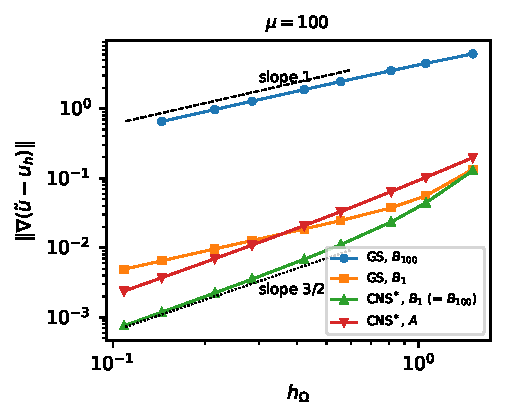
\includegraphics[width=0.48\textwidth]{figures/h1_rates.pdf}\hfill
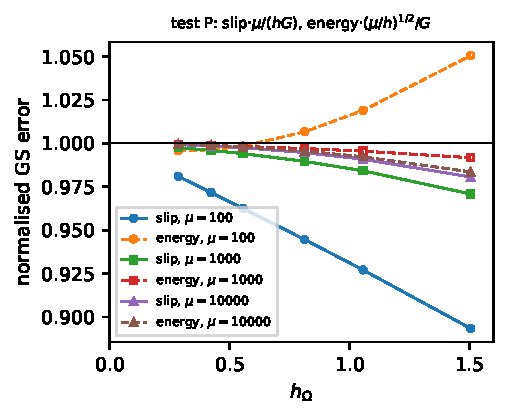
\includegraphics[width=0.48\textwidth]{figures/leading_term.pdf}
\caption{Left: $H^1$ errors at $\mu=100$. Once $G>0$, $\GS$ eventually has slope $1$, while $\CNS$ tends to slope $3/2$ independently of the pressure. Right: the normalised slip and energy errors of $\GS$ on test P approach $1$ (Corollary~\ref{cor:Bp}); at $N=96$ the energy ratios are within $0.5\%$ of $1$ and the slip ratios within $2\%$.}
\label{fig:rates}
\end{figure}

\begin{table}[t]
\centering
\caption{$\CNS$ attains Scott's rate $\hG^{3/2}$ (Theorem~\ref{thm:D}). $H^1$ error, $\mu=100$.}\label{tab:cns}
\begin{tabular}{rrcccc}
\toprule
$N$ & $\hO$ & A & rate & B$_1$ & rate\\
\midrule
32 & 0.813 & $6.41\cdot10^{-2}$ & 1.80 & $2.34\cdot10^{-2}$ & 2.43\\
64 & 0.422 & $2.08\cdot10^{-2}$ & 1.69 & $6.83\cdot10^{-3}$ & 1.76\\
96 & 0.285 & $1.09\cdot10^{-2}$ & 1.64 & $3.54\cdot10^{-3}$ & 1.68\\
128 & 0.215 & $6.96\cdot10^{-3}$ & 1.60 & $2.24\cdot10^{-3}$ & 1.63\\
192 & 0.144 & $3.71\cdot10^{-3}$ & 1.58 & $1.19\cdot10^{-3}$ & 1.60\\
256 & 0.109 & $2.39\cdot10^{-3}$ & 1.56 & $7.58\cdot10^{-4}$ & 1.57\\
\bottomrule
\end{tabular}
\end{table}

\subsection{Theorem~\ref{thm:D}: $\CNS$}
Table~\ref{tab:cns} gives the $\CNS$ errors. At $N=256$ the energy-norm rate is $1.52$ and the slip rate is $2.02$; the slip carries an extra factor $(h/\mu)^{1/2}$. The $H^1$ rates decrease monotonically toward $3/2$, the geometric term of Lemma~\ref{lem:transposed}. The $\hO^4$ term is invisible at these levels because the geometric term dominates.

The error is independent of the pressure.
\begin{itemize}
\item For polynomial pressures this is structural ($p\in\Pih$). B$_1$ and B$_{100}$ agree to all printed digits wherever both were run ($N\le192$, every $\mu$).
\item With the non-polynomial pressure of test C, the $\CNS$ $H^1$ error differs from that of B$_1$ by a relative $7.9\cdot10^{-7}$, $3.9\cdot10^{-8}$ and $9.7\cdot10^{-9}$ at $N=16$, $64$ and $96$. This is the size of the contribution $\ip{p^\ast-\pi_hp^\ast}{v\cdot n}$, which is of higher order, as Theorem~\ref{thm:D} predicts.
\end{itemize}

\subsection{Theorems~\ref{thm:A}--\ref{thm:C}: the printed method}
Table~\ref{tab:gs} compares the $H^1$ rates of $\GS$ and $\CNS$ on B$_{100}$.

For the non-polynomial test C at $\mu=100$, the $\GS$ $H^1$ rate from $N=64$ to $96$ is already $1.12$, against $1.68$ for $\CNS$. For the small pressure B$_1$ at $\mu=1000$, $\GS$ still shows $1.51$ at $N=192$. The $(h/\mu)G$ term dominates only once $(h/\mu)G\gtrsim\hG^{3/2}$, which always happens eventually because $\hG^{3/2}$ decays faster. Larger $\mu$ or smaller $G$ delays the crossover but does not remove it.

\begin{table}[t]
\centering
\caption{$\GS$ eventually loses Scott's rate once $G>0$. $H^1$ rate between $N=128$ and $N=192$, test B$_{100}$.}\label{tab:gs}
\begin{tabular}{rcc}
\toprule
$\mu$ & $\GS$ & $\CNS$\\
\midrule
100 & 0.99 & 1.60\\
1000 & 1.00 & 1.56\\
10000 & 1.06 & 1.58\\
\bottomrule
\end{tabular}
\end{table}

\subsection{Corollary~\ref{cor:Bp}: the leading term}
Table~\ref{tab:P} and Figure~\ref{fig:rates} (right) show the normalised $\GS$ error on test P, and Figure~\ref{fig:leak} shows the leak field itself.
\begin{itemize}
\item At $N=32$, $\mu=100$, the normal trace of $u_h$ on $\Gh$ matches the prediction $(h/\mu)(p-\pbar)$ with relative $L^2(\Gh)$ misfit $0.055$. The maximum of the tangential trace is about $12\%$ of that of the normal one, and the tangential trace oscillates at the element scale.
\item The slip and energy ratios approach $1$: at $N=96$ the energy ratios are within $0.5\%$ of $1$ for every $\mu$. The defect in the slip ratio shrinks with $h/\mu$: at $N=96$ it is $0.019$, $0.0025$ and $0.0007$ for $\mu=10^2$, $10^3$ and $10^4$.
\item The $H^1$ constant is not covered by the corollary. For $\mu=100$ it rises from $2.46$ to $2.71$; for $\mu=10^3$ and $10^4$ it falls, from $2.78$ to $2.77$ and from $3.06$ to $2.79$. Section~\ref{hc:sec} identifies the limit as $K=\norm{\nabla U}/G=2.7565$ for this box, proves convergence to it as $h\to0$ at fixed $\mu$ (Corollary~\ref{hc:cor}; on these meshes $h/\hG$ is nearly constant, so fixed $\mu$ means fixed $\gamma$ and bounded $\rho$), and compares it pointwise with these runs. The $\mu=100$ values approach it from below; the larger-$\mu$ values approach it from above, in a regime ($\gamma\hG\gg1$) that the proof does not cover (Remark~\ref{hc:regime}).
\item On test B, $\GS$ itself (B$_1$, $\mu=100$, $N=256$) gives slip and energy ratios $0.995$ and $1.001$.
\item For $\mu=10^4$ with the small pressure B$_1$, $\gamma\hG\approx120\gg G$ at $N=192$, so the hypothesis of the corollary fails. The $\GS$ energy ratio there is about $7.8$, dominated by the geometric error rather than the traction response.
\item The difference $u_{\GS}-u_{\CNS}$ is not a clean proxy for the traction response on test B. It also contains the difference between the two methods on the velocity part, which is $O(\hG^{3/2})$ and non-zero even for test A. Test P removes this.
\end{itemize}

\begin{figure}[t]
\centering
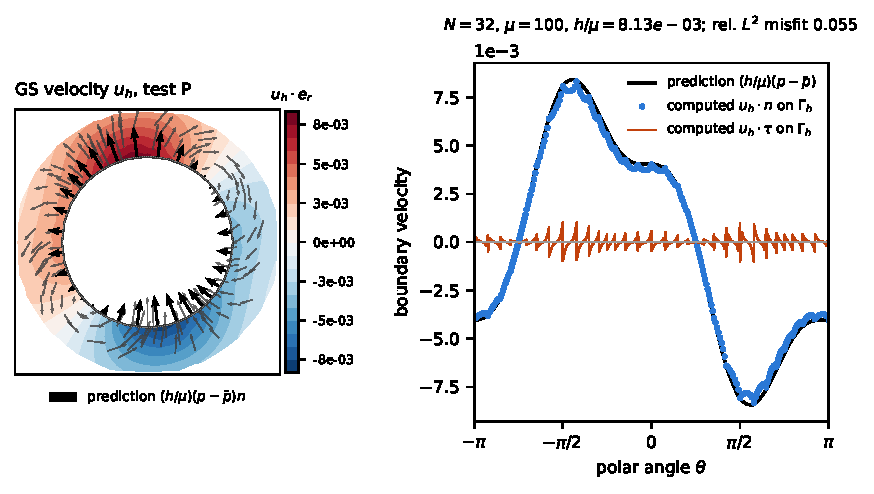
\includegraphics[width=\textwidth]{figures/leak_field.pdf}
\caption{The leak of the printed method on test P ($u=0$, so $u_h=-(\ut-u_h)$), $N=32$, $\mu=100$. Left: radial velocity $u_h\cdot e_r$ near the wall (colour) and $u_h$ (thin arrows); thick arrows show the prediction $(h/\mu)(p-\pbar)n$ of Corollary~\ref{cor:Bp} at the chord midpoints. Right: normal and tangential traces of $u_h$ along $\Gh$ against $(h/\mu)(p-\pbar)$.}
\label{fig:leak}
\end{figure}

\begin{table}[t]
\centering
\caption{The leading term of Corollary~\ref{cor:Bp}. Normalised $\GS$ error on test P ($G=1.658$), where $e=\ut-u_h$.}\label{tab:P}
\begin{tabular}{rrccc}
\toprule
$N$ & $\mu$ & $\norm{\nabla e}\,\mu/(hG)$ & $\norm{e}_{\Gh}\,\mu/(hG)$ & $\tnorm{e}(\mu/h)^{1/2}/G$\\
\midrule
16 & 100 & 2.464 & 0.893 & 1.050\\
32 & 100 & 2.612 & 0.945 & 1.007\\
64 & 100 & 2.684 & 0.972 & 0.996\\
96 & 100 & 2.708 & 0.981 & 0.996\\
96 & 1000 & 2.770 & 0.998 & 0.999\\
96 & 10000 & 2.790 & 0.9993 & 0.9994\\
\bottomrule
\end{tabular}
\end{table}

\subsection{Proposition~\ref{prop:penalty}: the penalty study}
The coercivity threshold $\mu^\ast$ on $\Zh$ is the smallest $\mu$ for which the unpivoted symmetric factorisation of $A_\mu+rB^{\mathsf T}M^{-1}B$ has only positive pivots; we locate it by bisection. Table~\ref{tab:thresh} and Figure~\ref{fig:thresh} show the results.

Under refinement at fixed $h/\hG$, $\gamma^\ast$ increases by $3.4$ ($N=8\to16$), $1.8$ ($16\to32$) and $0.95$ ($32\to64$). The increments roughly halve. The patch computations of Section~\ref{pb:sec} (limit geometry, windows of up to $32$ boundary edges) predict a limit $\gamma^\ast_\infty\approx21.4$; this is an extrapolation, not a proof.

In part (b) of Table~\ref{tab:thresh}, $h/\hG$ is varied by coarsening the far field while the vertices of $\Gh$ are held fixed and the boundary layer approximately fixed. Then $\mu^\ast$ is linear in $h/\hG$ over more than a decade, with a constant slope of about $18$--$20$. The vertices of $\Gh$ do not depend on $L$, so $\max|e|/\min|e|$ is fixed at fixed $N$, and $\mu^\ast$ is equally linear in $\rho$, with the slope divided by that ratio. The threshold is thus set locally at $\Gh$ ($\mu/h\gtrsim c/\hG$), and the scaling with $h/\hG$ (hence with $\rho$) is the cost of normalising the penalty by the global $h$.

In practical terms:
\begin{itemize}
\item for $k=4$ a safe choice is $\gamma=\mu\hG/h\ge25$, that is, $\mu\ge25\,h/\hG$; since $\rho\ge h/\hG$, $\mu\ge25\rho$ is also safe;
\item a fixed $\mu$ fails once the far field is coarsened beyond $h/\hG\approx\mu/20$;
\item the threshold grows quickly with $k$, and is larger on Clough--Tocher refinements (Section~\ref{sec:numv3}), so these values do not transfer to other elements.
\end{itemize}
The exact certificate $\lambda\ge9$ on $\cS_3$ and $\cS_4'$ is a local lower bound, consistent with the global $\gamma^\ast\approx18$--$21$; Section~\ref{pb:sec} accounts for the gap.

\begin{table}[t]
\centering
\caption{Coercivity threshold $\mu^\ast$ and $\gamma^\ast=\mu^\ast\hG/h$ ($k=4$). The row $h/\hG$ is $\hO/\max|e|$; the $\rho=h/\min|e|$ of Section~\ref{sec:setting} is larger by the factor $\max|e|/\min|e|$ (for example $\rho=4.70$, $5.73$, $6.35$ at $N=16$, $32$, $64$ in part (a)).}\label{tab:thresh}
\small
\textit{(a) Refinement at fixed $h/\hG\approx3.3$.}\\[2pt]
\begin{tabular}{lcccccccc}
\toprule
$N$ & 8 & 12 & 16 & 20 & 24 & 32 & 48 & 64\\
\midrule
$h/\hG$ & 3.41 & 3.02 & 3.28 & 3.17 & 3.30 & 3.33 & 3.37 & 3.40\\
$\mu^\ast$ & 50.3 & 51.8 & 59.3 & 60.3 & 63.3 & 66.0 & 69.1 & 70.7\\
$\gamma^\ast$ & 14.7 & 17.1 & 18.1 & 19.1 & 19.2 & 19.9 & 20.5 & 20.8\\
\bottomrule
\end{tabular}\\[6pt]
\textit{(b) Varying $h/\hG$ through the outer box $(-L,L)^2$.}\\[2pt]
\begin{tabular}{llccccc}
\toprule
 & $L$ & 2.5 & 5 & 10 & 20 & 40\\
\midrule
$N=16$ & $h/\hG$ & 3.28 & 5.90 & 11.3 & 22.2 & 43.9\\
 & $\mu^\ast$ & 59.3 & 112.1 & 208.0 & 411.5 & 809.3\\
 & $\gamma^\ast$ & 18.1 & 19.0 & 18.4 & 18.5 & 18.4\\
\midrule
$N=32$ & $h/\hG$ & 3.33 & 5.79 & 10.8 & 21.1 & 41.5\\
 & $\mu^\ast$ & 66.0 & 113.9 & 218.0 & 422.2 & 835.7\\
 & $\gamma^\ast$ & 19.9 & 19.7 & 20.1 & 20.0 & 20.1\\
\bottomrule
\end{tabular}
\end{table}

\begin{figure}[t]
\centering
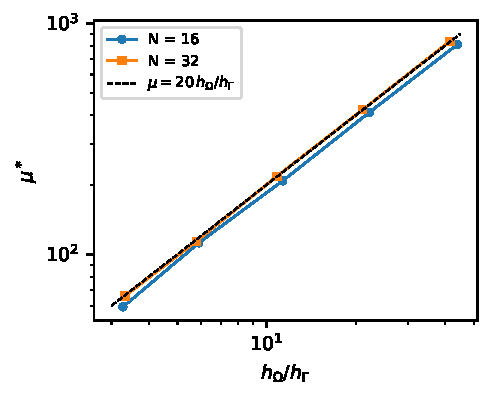
\includegraphics[width=0.48\textwidth]{figures/threshold.pdf}
\caption{Coercivity threshold $\mu^\ast$ against $h/\hG$ (Table~\ref{tab:thresh}(b)).}
\label{fig:thresh}
\end{figure}

\subsection{Lemma tests}
We compute exact discrete dual norms, $\sup_v\ell(v)/\norm{\nabla v}$ over $\Zh$ or $\VR$, by a saddle-point solve with the pointwise divergence constraint. Table~\ref{tab:lemma} gives the rates for $N=48\to64$.
\cert{code/lemma\_tests.py 16,24,32,48,64}{logs/lemma\_tests.log}

\begin{table}[t]
\centering
\caption{Exact discrete dual norms; rate in $\hG$ for $N=48\to64$ (positive means decay).}\label{tab:lemma}
\begin{tabular}{llc}
\toprule
Functional & Space & Rate\\
\midrule
$\ip{S}{\dn v}$, $S$ normal & $\Zh$ & $+0.05$ (bounded, $\approx1.75$)\\
$\ip{S}{\dn v}$, $S$ normal & $\VR$ & $-0.52$\\
$\ip{S}{\dn v}$, $S$ tangential & $\Zh$ & $-0.52$\\
$\ip{(\nabla\ut)^{\mathsf T}n}{v}$, tests A / B & $\VR$ & $1.57$ / $1.56$ (Lemma~\ref{lem:transposed}: $3/2$)\\
\bottomrule
\end{tabular}
\end{table}

\subsection{Higher degree and Clough--Tocher refinements}\label{sec:numv3}
We repeated the study with $k=5,6$ on the same meshes, and with $k=2,3$ on their Clough--Tocher refinements (Section~\ref{ct:sec}), using a degree-general version of the solver (\texttt{code/svn\_k.py}). The refinement leaves $\Gh$, the square and $h=\hO$ unchanged, so the $h$ values are those of the standard meshes. At $k=4$ with SuperLU the new code is bit-identical to \texttt{svn.py}, and agrees with the stored production records to $2.6\cdot10^{-10}$ relative. SuperLU runs out of memory at the target sizes, so these runs use MKL PARDISO. The saddle-point matrix is ill-conditioned, and for robustness of PARDISO we regularise the pressure block by $10^{-12}$ times the pressure mass matrix. The result agrees with SuperLU to $\le10^{-9}$ relative ($k=4$ and $k=6$, $N\le32$). Over the $260$ solves ($390$ records, including $130$ derived records for $D$) the relative residual of the unregularised system is at most $2.2\cdot10^{-12}$ and the discrete divergence at most $10^{-9}$. One side effect: $\CNS$ on test P returns $\norm{\nabla u_h}\approx4\cdot10^{-11}$, the regularisation floor, instead of round-off.

\emph{Thresholds.} Table~\ref{tab:threshv3} gives $\gamma^\ast$. It grows quickly with $k$ and is larger on the Clough--Tocher refinements, whose boundary triangles are three times thinner while $h$ is the macro size. In every case the measured value exceeds the corresponding certified local constant (Proposition~\ref{prop:penalty} for $k\ge4$, Proposition~\ref{ct:prop:penalty} on the refinements), which is consistent with those constants being local lower bounds. $\gamma^\ast$ still drifts upward with $N$ ($+7\%$ to $+24\%$ from $N=16$ to $64$). In particular $\mu=100$ is \emph{below} the threshold for $k=5$ ($N\ge32$), for $k=6$ and for Clough--Tocher $k=3$ (all $N$). The $\mu=100$ runs in those cases are erratic, as they should be (for instance the $\CNS$ $H^1$ error for $k=5$ on B$_1$ jumps between $0.05$ and $3.7$), and they are not covered by the theory. We therefore report $\mu=300$ and $\mu=1000$ for them.

\begin{table}[t]
\centering
\caption{Coercivity threshold $\gamma^\ast=\mu^\ast\hG/h$ for higher degrees and on Clough--Tocher (CT) refinements. The $k=4$ row is Table~\ref{tab:thresh}(a).}\label{tab:threshv3}
\begin{tabular}{lccccc}
\toprule
 & $N=8$ & $16$ & $32$ & $64$ & $128$\\
\midrule
$k=4$ & 14.7 & 18.1 & 19.9 & 20.8 & --\\
$k=5$ & 25.7 & 30.3 & 32.1 & 33.0 & --\\
$k=6$ & -- & 45.2 & 47.4 & 48.3 & --\\
CT, $k=2$ & 5.7 & 9.1 & 10.5 & 11.2 & 11.5\\
CT, $k=3$ & -- & 31.6 & 33.9 & 34.6 & --\\
CT, $k=4$ & -- & 61.9 & 65.5 & -- & --\\
\bottomrule
\end{tabular}
\end{table}

\emph{The leak (test P).} Table~\ref{tab:Pv3} shows that the slip and energy constants of Corollary~\ref{cor:Bp} tend to $1$ for every element, with rates $1$ (slip), $1/2$ (energy) and $1$ ($H^1$). The $H^1$ constants are close to the $K=2.7565$ of Section~\ref{hc:sec}, which does not depend on the element; this agreement is observed, not proved, for these elements. On test B$_1$ the leak part $D:=u_{\GS}-u_{\CNS}$ has the same normalised slip and energy ratios ($0.986$--$1.003$ and $0.991$--$1.006$ at the finest levels), $H^1$ rate $1.01$--$1.15$ and energy rate $0.49$--$0.52$. Its normalised $H^1$ constant is still drifting down at the finest levels ($3.03$ for $k=5$, $\mu=1000$).

\begin{table}[t]
\centering
\caption{Normalised $\GS$ error on test P at the finest level run, $e=\ut-u_h$.}\label{tab:Pv3}
\begin{tabular}{lrrccc}
\toprule
Element & $\mu$ & $N$ & $\norm{\nabla e}\,\mu/(hG)$ & $\norm{e}_{\Gh}\,\mu/(hG)$ & $\tnorm{e}(\mu/h)^{1/2}/G$\\
\midrule
$k=4$ & 1000 & 96 & 2.770 & 0.998 & 0.999\\
$k=5$ & 1000 & 128 & 2.768 & 0.9983 & 0.9994\\
$k=6$ & 1000 & 96 & 2.769 & 0.9976 & 0.9993\\
CT, $k=2$ & 100 & 256 & 2.737 & 0.9928 & 0.9974\\
CT, $k=2$ & 1000 & 128 & 2.751 & 0.9982 & 0.9992\\
CT, $k=3$ & 1000 & 128 & 2.763 & 0.9983 & 0.9996\\
\bottomrule
\end{tabular}
\end{table}

\emph{Rates.} Table~\ref{tab:ratesv3} gives $H^1$ rates at the finest pair of levels.
\begin{itemize}
\item \emph{$\CNS$ tends to rate $3/2$} for $k=5,6$ on B$_1$ ($1.58$--$1.61$, energy rate $1.53$--$1.54$), non-increasing from $N=32$ on. The $\CNS$ errors for $k=4,5,6$ are almost equal (for example $1.05\cdot10^{-2}$, $9.02\cdot10^{-3}$, $8.47\cdot10^{-3}$ at $N=64$, $\mu=1000$): the geometric term dominates. On Clough--Tocher $k=3$, test A, the $H^1$ rate is $1.56$ at $N=128$.
\item \emph{$\GS$ tends to rate $1$ when $G>0$.} For $k=5$, $\mu=300$, the $\GS$ $H^1$ rate on B$_1$ decreases monotonically, $1.63,1.58,1.48,1.38,1.28,1.20$ for $N=24,\dots,128$, while its leak part $D$ already has rate $1.03$. At $\mu=1000$ the crossover comes later ($1.53$ at $N=128$), exactly as for $k=4$.
\item \emph{$\CNS$ is pressure-independent} for $k=5,6$: on test P it returns $u_h=0$ to the regularisation floor at every $N$ and every $\mu\ge\mu^\ast$. By linearity this is the statement that $u_h(\mathrm B_a)=u_h(\mathrm B_1)$ for every $a$.
\end{itemize}

\begin{table}[t]
\centering
\caption{$H^1$ rates at the finest pair of levels (energy-norm rate of $\CNS$ in parentheses). $D=u_{\GS}-u_{\CNS}$ is the leak part; it is not reported for test A, where $G=0$.}\label{tab:ratesv3}
\begin{tabular}{llrrccc}
\toprule
Element & Test & $\mu$ & $N$ & $\GS$ & $\CNS$ & $D$\\
\midrule
$k=5$ & B$_1$ & 300 & $96\to128$ & 1.20 & 1.59 (1.53) & 1.03\\
$k=5$ & B$_1$ & 1000 & $96\to128$ & 1.53 & 1.58 (1.54) & 1.13\\
$k=6$ & B$_1$ & 300 & $64\to96$ & 1.27 & 1.61 (1.54) & 1.04\\
$k=6$ & B$_1$ & 1000 & $64\to96$ & 1.57 & 1.61 (1.54) & 1.15\\
CT, $k=3$ & A & 1000 & $96\to128$ & 1.56 & 1.56 (1.55) & --\\
CT, $k=2$ & A & 100 & $192\to256$ & 1.78 & 1.78 (1.55) & --\\
CT, $k=2$ & B$_1$ & 100 & $192\to256$ & 1.91 & 1.91 (1.91) & 1.01\\
CT, $k=3$ & B$_1$ & 1000 & $96\to128$ & 2.83 & 2.83 (1.64) & 1.05\\
\bottomrule
\end{tabular}
\end{table}

\emph{Caveats for Clough--Tocher $k=2,3$.}
\begin{enumerate}
\item \emph{$\CNS$ on test P is not exactly zero.} The pressure $p=x^2y-y+x/2$ is cubic, so $p\notin\Pih$ for $k\le3$, and the term $\eta=p^\ast-\pi_hp^\ast$ of Theorem~\ref{thm:D} is present. The spurious velocity is small and converges at a rate close to $k+\frac12$: $\norm{\nabla u_h}=1.4\cdot10^{-6}$ at $N=256$ for $k=2$ (rate $2.56$), and $4.7\cdot10^{-9}$ at $N=128$ for $k=3$ (rate $3.53$). So for $k\le3$ the pressure-independence of $\CNS$ holds only up to a term of order $h^{k+1/2}$ that scales with the amplitude of $p$. It is below $\hG^{3/2}$ asymptotically, but for B$_{100}$ it would be $100$ times larger.
\item \emph{On test B$_1$ the rate $3/2$ is not yet visible.} The $H^1$ error is dominated by interpolation of the steep velocity ($u$ grows like $r^5$, since $\psi$ grows like $r^6$, on the square of side $5$): for $k=2$ it is $0.41$ at $N=256$, against $7.6\cdot10^{-4}$ for $k=4$, with rate $1.91$ still rising towards $2$. For $k=3$ the rate is $2.83$, close to $3$. The runs are pre-asymptotic and the crossover to $\hG^{3/2}$ is out of reach. The leak part $D$ is on theory (rate $1.01$, ratios $1.0009$ and $1.0056$ at $N=256$ for $k=2$).
\item On test A (bounded velocity) the energy-norm rate is already $1.55$ for $k=2$, while the $H^1$ rate ($1.78$ at $N=256$) is still decreasing.
\end{enumerate}
Memory limits (a shared 5.8\,GB budget) prevented $k=6$ at $N=128$ and Clough--Tocher $k=3$ at $N=192$.
